\markright{Implementation}
\section{Implementation}
\label{Implementation}
\definecolor{lightgray}{gray}{0.93}
  \vskip\baselineskip%
  \par\noindent\colorbox{lightgray}{%
    \begin{minipage}{0.98\textwidth}
		\textsc{Source Code}:\\
		The extended and working version of the code presented in this paper can be found on:\\
		\texttt{https://github.com/thoeni/rtos-project.git}
		\\There are two branches, the \texttt{main} and the \texttt{icecream} (which has been tested on \texttt{Android 4.0.1\_r1})
    \end{minipage}%
  }%
  \vskip\baselineskip%
As shortly described in the previous section, this small example relies on a native library we'll implement, and a summary of the flow from the Client Application (Activity named BbqueActivity) to the Server (Daemon named bbqued) can be seen in Fig. \ref{fig:projectoverview}.
\begin{figure}[!htb]
	\centering
	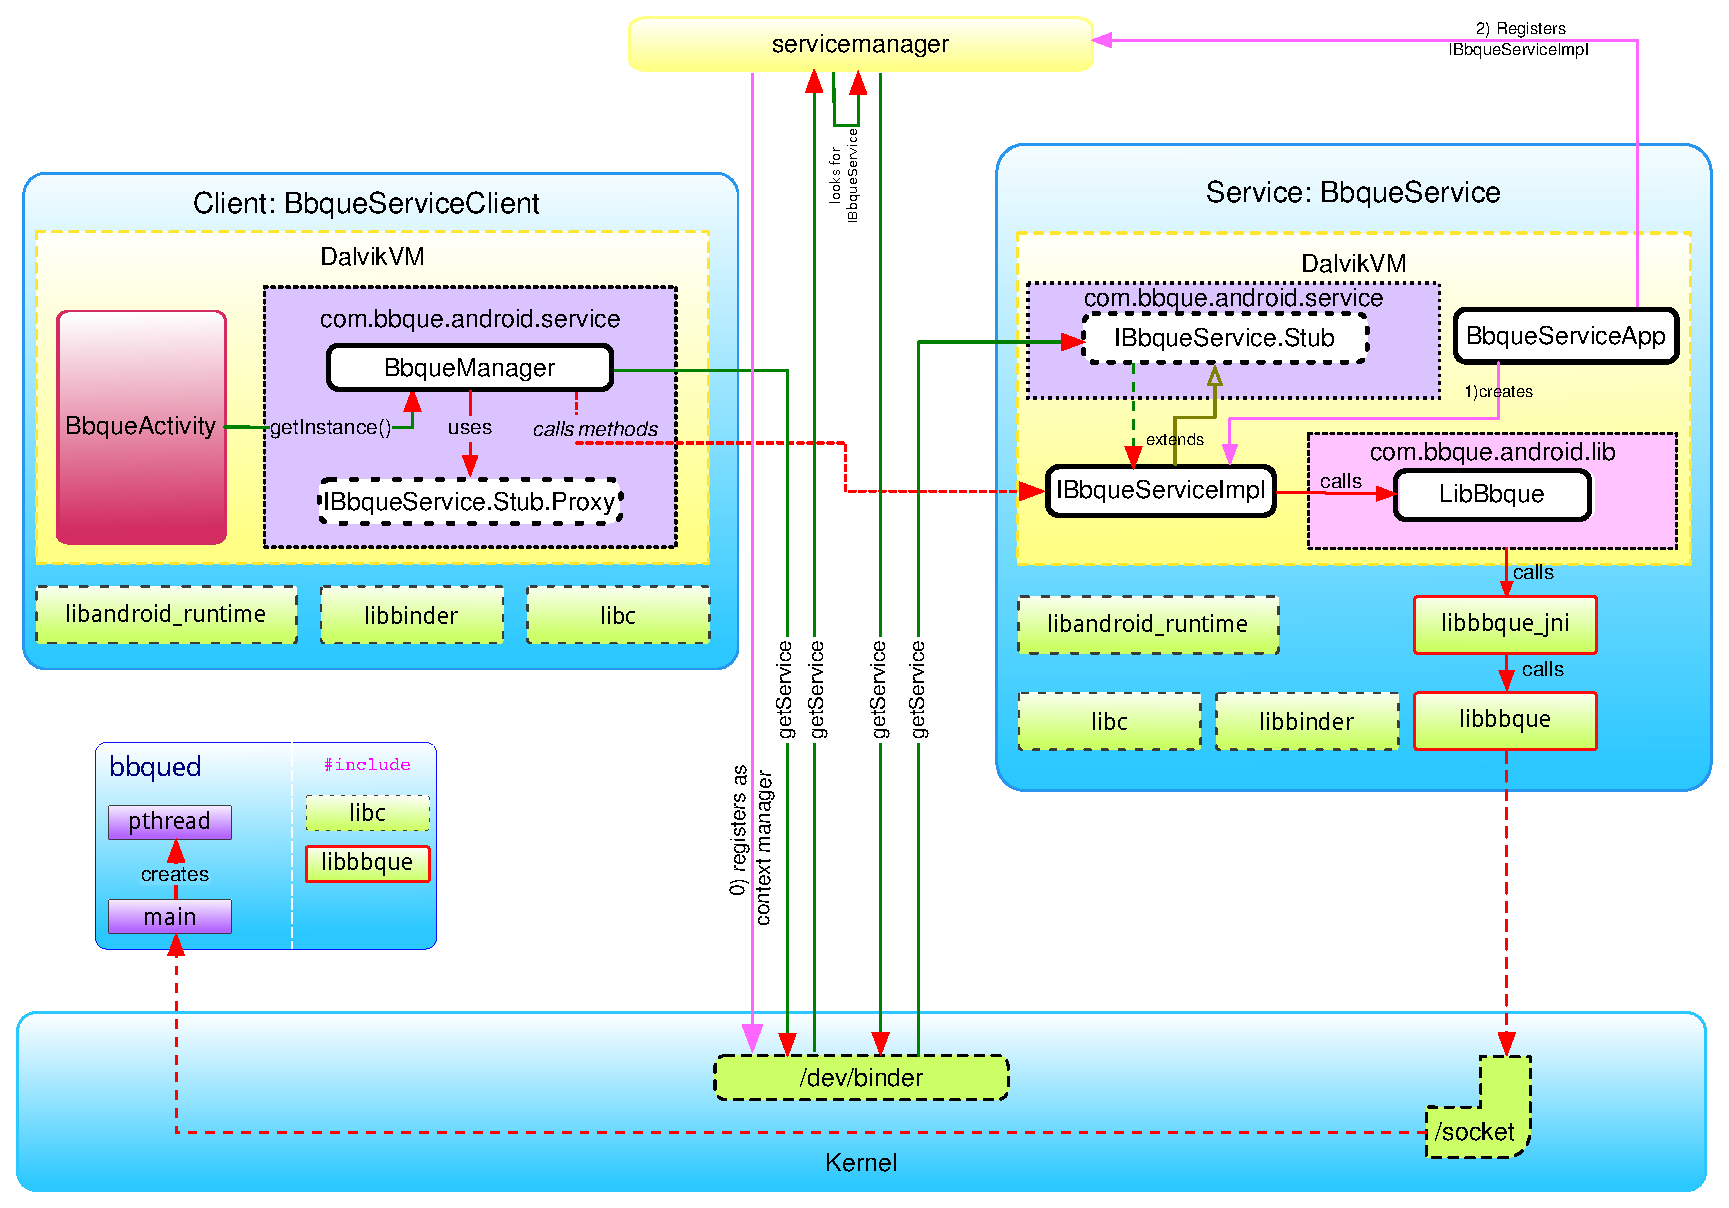
\includegraphics[scale=.432]{images/project_overview.pdf}
	\caption{Project flow overview}
	\label{fig:projectoverview}
\end{figure} 